\documentclass[12pt]{scrartcl}

\setlength{\parindent}{0pt}
\setlength{\parskip}{.25cm}

\usepackage{graphicx}

\usepackage{xcolor}

\definecolor{darkred}{rgb}{0.5,0,0}
\definecolor{darkgreen}{rgb}{0,0.5,0}
\usepackage{hyperref}
\hypersetup{
  letterpaper,
  colorlinks,
  linkcolor=red,
  citecolor=darkgreen,
  menucolor=darkred,
  urlcolor=blue,
  pdfpagemode=none,
  pdftitle={CSCE 156 Lab Handout},
  pdfsubject={},
  pdfkeywords={}
}

\definecolor{MyDarkBlue}{rgb}{0,0.08,0.45}
\definecolor{MyDarkRed}{rgb}{0.45,0.08,0}
\definecolor{MyDarkGreen}{rgb}{0.08,0.45,0.08}

\definecolor{mintedBackground}{rgb}{0.95,0.95,0.95}
\definecolor{mintedInlineBackground}{rgb}{.90,.90,1}

%\usepackage{newfloat}
\usepackage[newfloat=true]{minted}
\setminted{mathescape,
               linenos,
               autogobble,
               frame=none,
               framesep=2mm,
               framerule=0.4pt,
               %label=foo,
               xleftmargin=2em,
               xrightmargin=0em,
               startinline=true,  %PHP only, allow it to omit the PHP Tags *** with this option, variables using dollar sign in comments are treated as latex math
               numbersep=10pt, %gap between line numbers and start of line
               style=default, %syntax highlighting style, default is "default"
               			    %gallery: http://help.farbox.com/pygments.html
			    	    %list available: pygmentize -L styles
               bgcolor=mintedBackground} %prevents breaking across pages
               
\setmintedinline{bgcolor={mintedBackground}}
\setminted[text]{bgcolor={mintedBackground},linenos=false,autogobble,xleftmargin=1em}
%\setminted[php]{bgcolor=mintedBackgroundPHP} %startinline=True}
\SetupFloatingEnvironment{listing}{name=Code Sample}
\SetupFloatingEnvironment{listing}{listname=List of Code Samples}

\title{CSCE 156 -- Computer Science II}
\subtitle{Lab 1.0 - Introduction}
\author{~}
\date{~}

\begin{document}

\maketitle

\section*{Prior to Lab}

In each lab there may be pre-lab activities that you are \emph{required} to
complete prior to attending lab.  Failure to do so may mean that you will
not be given full credit for the lab.  For the first lab, there are no pre-lab
activities.

\section{Lab Objectives \& Topics}
Following the lab, you should be able to:
\begin{itemize}
  \item Receive and activate your CSE account and log into the network 
  	using a Windows machine and your CSE account.
  \item Clone projects from GitHub using Eclipse
  \item Open, compile, and execute a given Java program in Eclipse.
  \item Write a simple program in the selected IDE, compile, and 
  	execute that program.
\end{itemize}

\section*{Peer Programming Pair-Up}

To encourage collaboration and a team environment, labs will be
structured in a \emph{pair programming} setup.  At the start of
each lab, you will be randomly paired up with another student 
(conflicts such as absences will be dealt with by the lab instructor).
One of you will be designated the \emph{driver} and the other
the \emph{navigator}.  

The navigator will be responsible for reading the instructions and
telling the driver what to do next.  The driver will be in charge of the
keyboard and workstation.  Both driver and navigator are responsible
for suggesting fixes and solutions together.  Neither the navigator
nor the driver is ``in charge.''  Beyond your immediate pairing, you
are encouraged to help and interact and with other pairs in the lab.

Each week you should alternate: if you were a driver last week, 
be a navigator next, etc.  Resolve any issues (you were both drivers
last week) within your pair.  Ask the lab instructor to resolve issues
only when you cannot come to a consensus.  

Because of the peer programming setup of labs, it is absolutely 
essential that you complete any pre-lab activities and familiarize
yourself with the handouts prior to coming to lab.  Failure to do
so will negatively impact your ability to collaborate and work with 
others which may mean that you will not be able to complete the
lab.  

\section{Getting Started}

\subsection{Login \& Consent Form}

If you do not already have a CSE login, you will receive one from 
the CSE System Administrators who will also give you an overview 
of the CSE system and its policies.  Be sure to login and 
change your temporary password.  Some departmental resources 
that you may find useful:
\begin{itemize}
  \item CSE Website: \url{http://cse.unl.edu}
  \item UNL Computing Policy: \url{http://www.unl.edu/ucomm/compuse/}
   \item CSE Academic Integrity Policy: \url{http://cse.unl.edu/academic-integrity-policy}
   \item CSE System FAQ: \url{http://cse.unl.edu/faq}
   \item Account Management: \url{https://cse-apps.unl.edu/amu/}
   \item CSE Undergraduate Advising Page: \url{http://cse.unl.edu/advising}
   \item CSE Student Resource Center: \url{http://cse.unl.edu/src}
\end{itemize}

\subsection{Checking Out Code From Github Using Eclipse}

Each lab will have some starter code and other \emph{artifacts} (data files, 
scripts, etc.) that will be provided for to you.  The code is hosted
on Github (\url{https://github.com}) and you must clone your own copy
to work with it.  You will not need to know the details of using git 
nor be a registered Github user to get access to the code necessary 
for your labs.  However, you are \emph{highly encouraged} to learn 
this essential tool.  You may find it very useful to keep track of your 
own code and to share code if you work in pairs or groups.  

Eclipse is the de facto industry-standard IDE for Java development.  There
are several other popular and emerging IDEs available and you are welcome
(and encouraged) to try them out and use them.  However, for this course, we
will primarily use Eclipse.

To check out the code for this lab, do the following.  You may want
to reference this step-by-step process in subsequent labs.

\begin{enumerate}
  \item First we need a Git \emph{perspective} (a context in the Eclipse User Interface that 
  	will allow us to work with Git).  To open the Git perspective, click on the ``Open Perspective''
	tab in the upper right:
	\begin{center}
	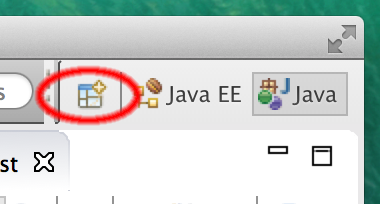
\includegraphics[scale=0.50]{images/eclipseOpenPerspectiveMarkUp}
	\end{center}
	Select ``Git'' from the menu and click OK
  \item Click the ``Clone a Git repository'' in the Git Repositories navigation menu:
  	\begin{center}
	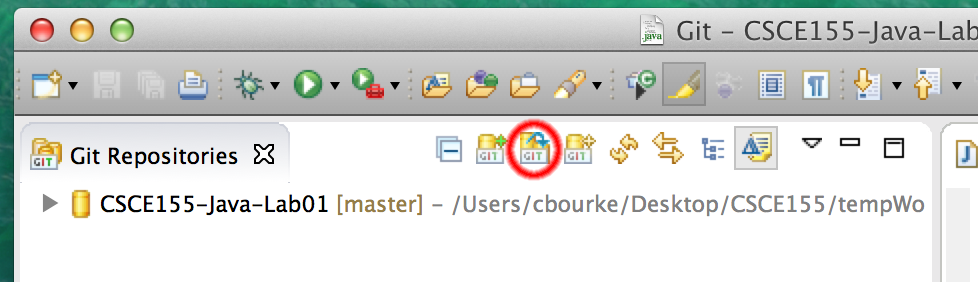
\includegraphics[scale=0.50]{images/eclipseGitRepoMarkUp}
	\end{center}
  \item Copy/past or type into the URI field, the URL: \\
  	\url{https://github.com/cbourke/CSCE156-Lab01}
  	\begin{center}
	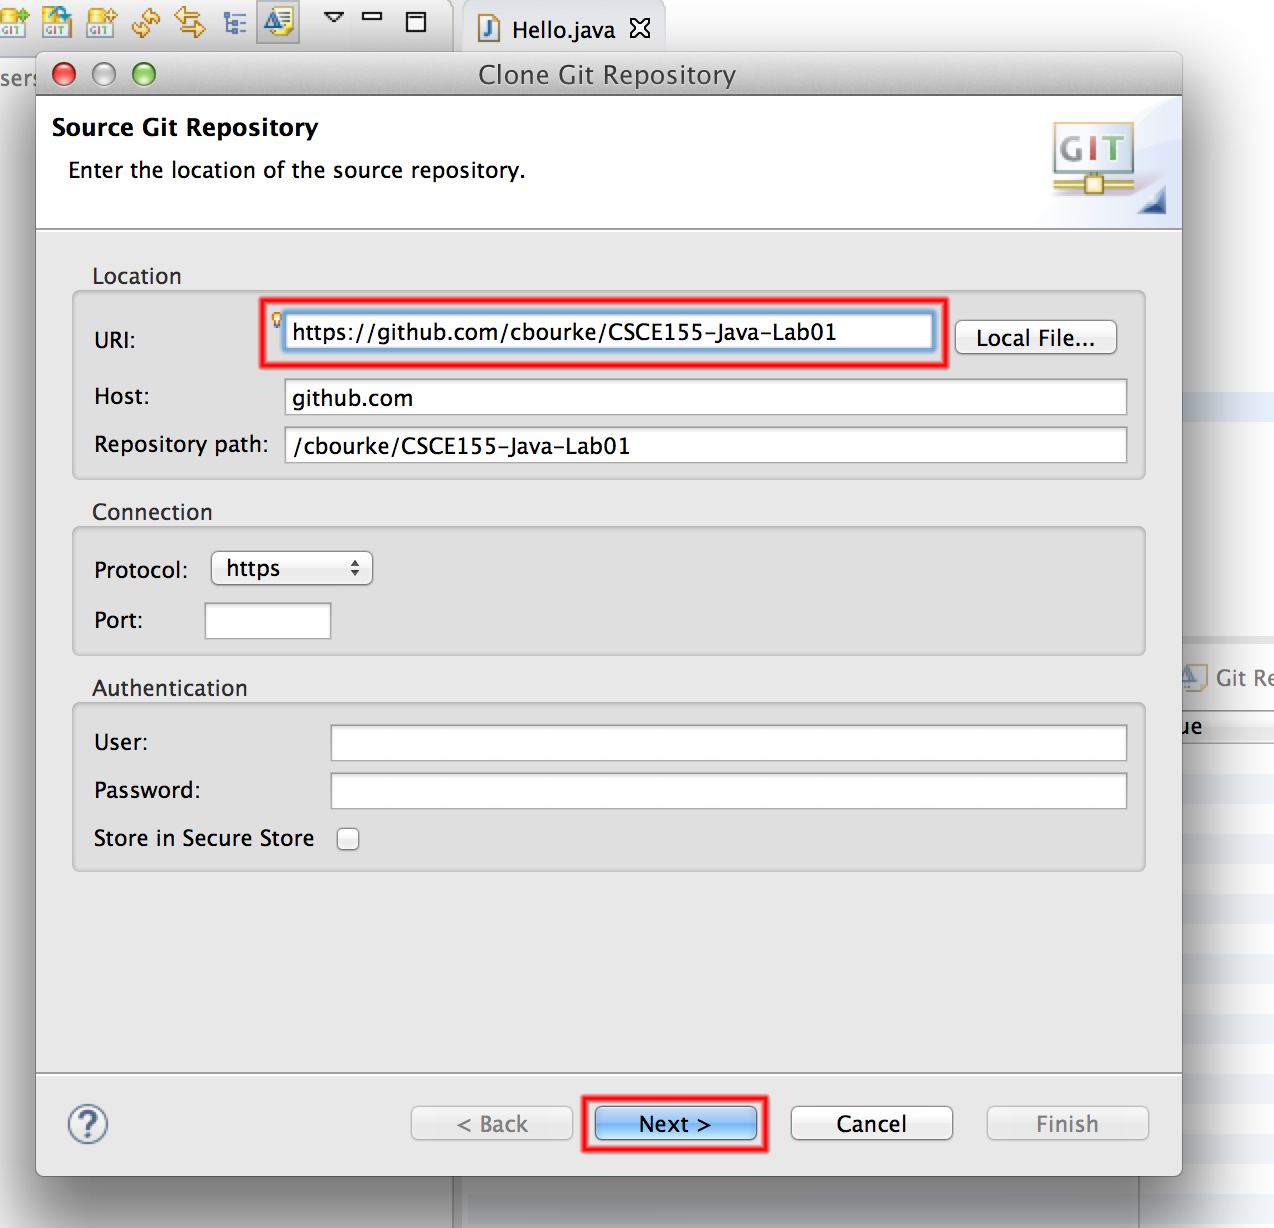
\includegraphics[scale=0.35]{images/eclipseCloneDialogAMarkUp}
	\end{center}
  \item Click ``Next''; once Eclipse has grabbed the project, the ``master'' branch should
  	be selected (checkbox); click ``Next'' again.
  	\begin{center}
	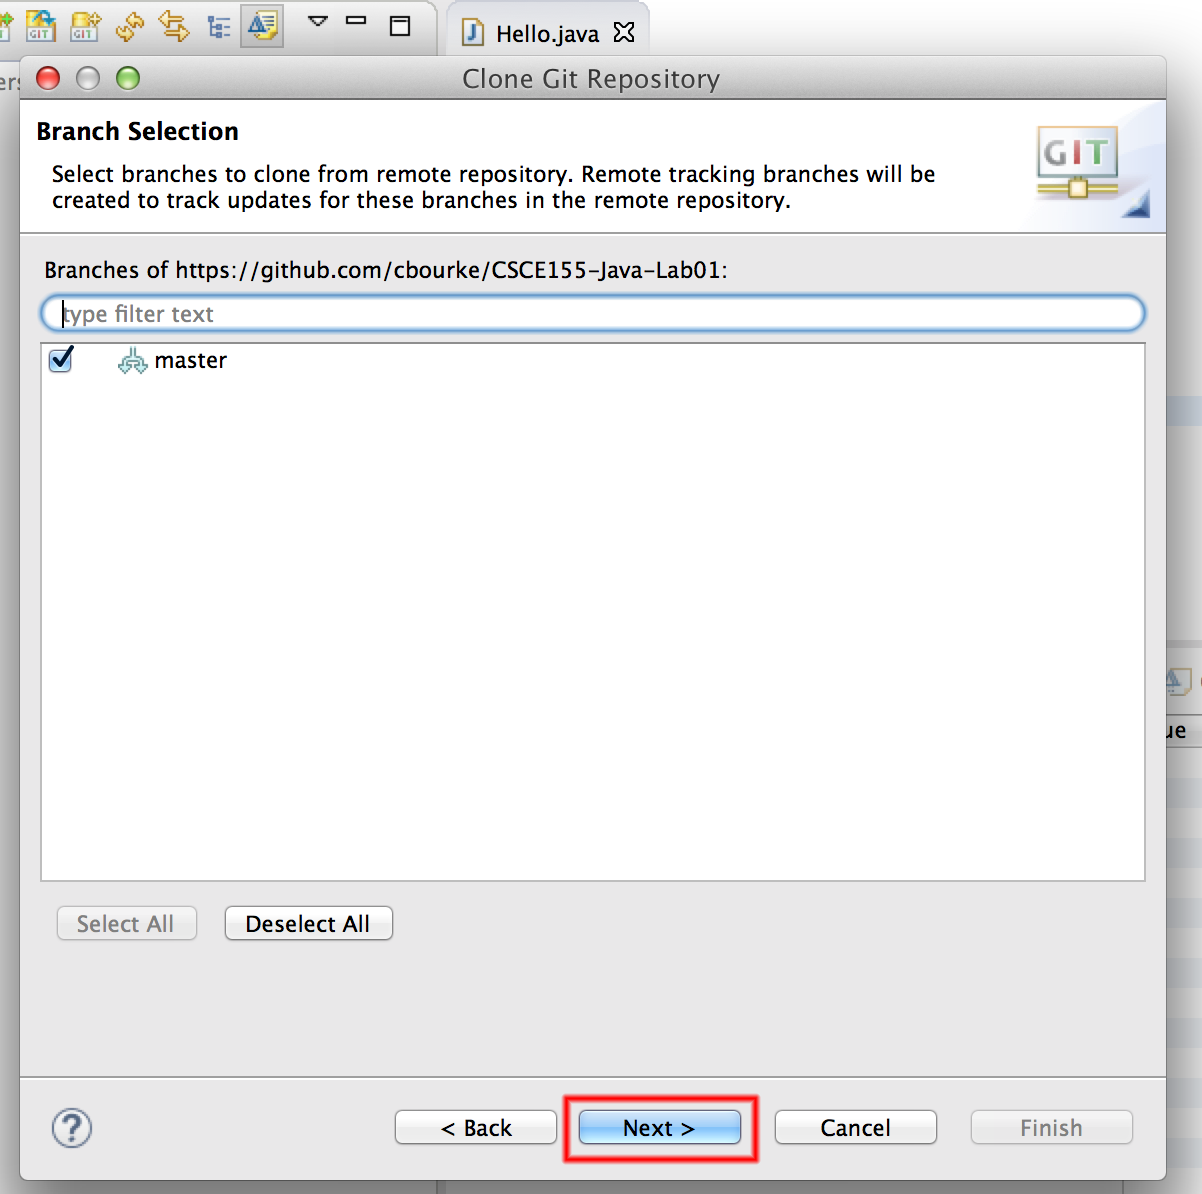
\includegraphics[scale=0.35]{images/eclipseCloneDialogBMarkUp}
	\end{center}
  \item Select the directory where you want your project to be saved.  Caution: the default
  	option may not correspond to your default workspace.  You may want to change
	it to your workspace, but the choice is yours.  Also mark the ``Import all existing 
	projects after clone finishes'' checkbox option or you will need
  	to manually import the cloned project into Eclipse.
  	\begin{center}
	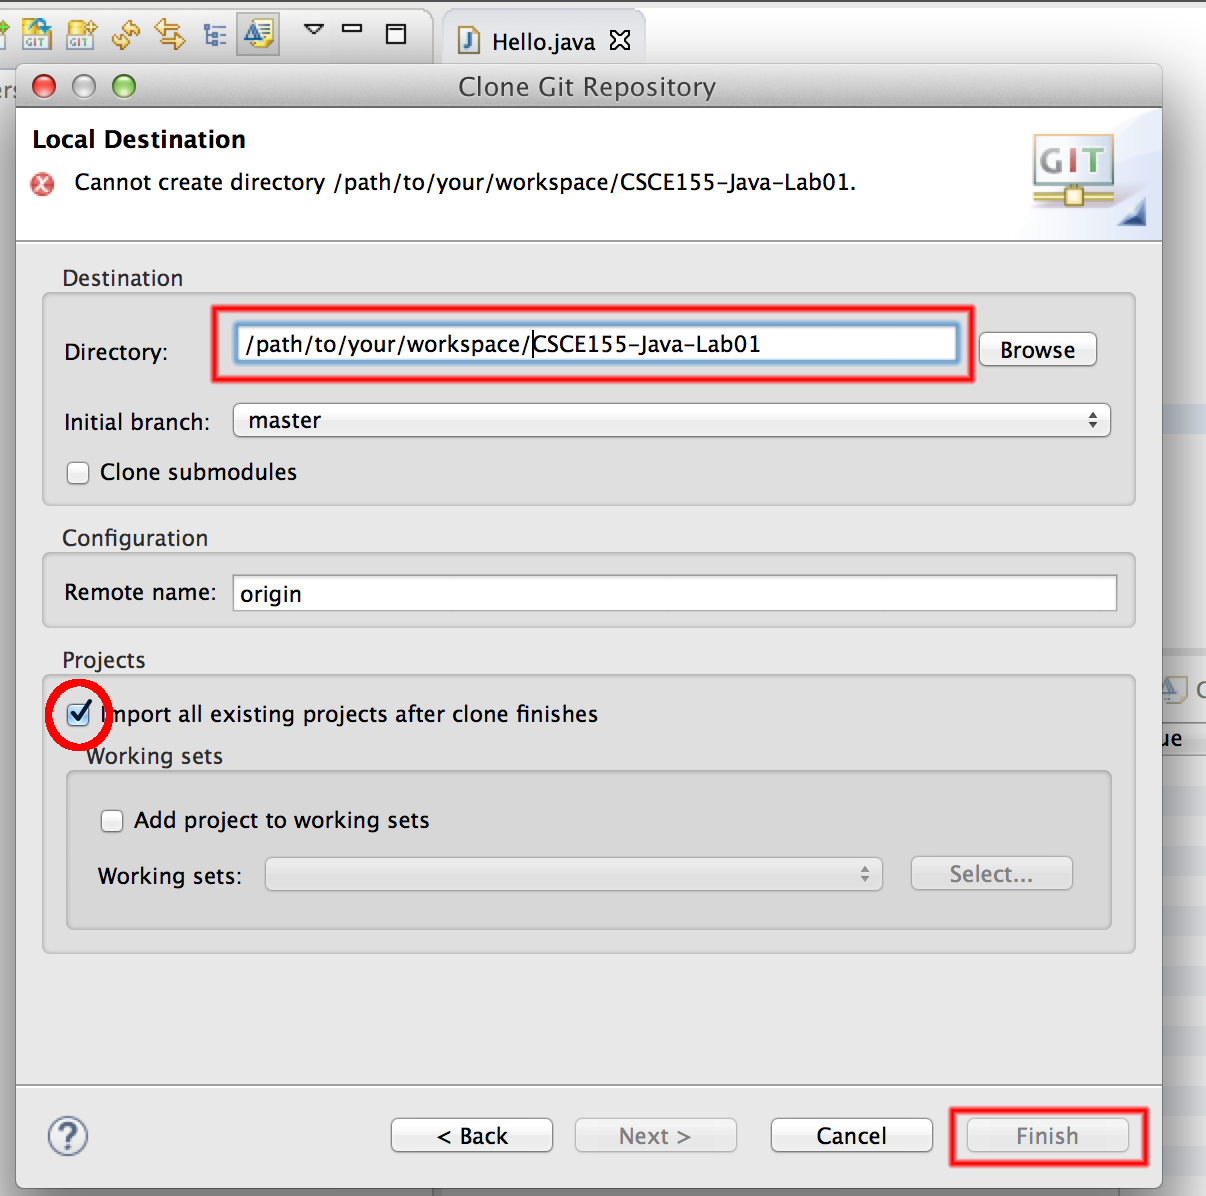
\includegraphics[scale=0.35]{images/eclipseCloneDialogCMarkUp}
	\end{center}
  \item Switch back to your Java or JavaEE perspective and you can see 
  	your cloned project.  
\end{enumerate}

Note: this process assumes that the project you are cloning originated 
from an Eclipse project.  Eclipse expects that files be organized in a particular way and that configuration files are present that describe 
how the project is setup.  If the project was not an Eclipse project, 
you'll need to clone/setup the project in Eclipse manually.

{\color{red}{\textbf{Note:}}} To complete the Java version of this lab proceed to 
section \ref{section:javaPart}; to complete the PHP version of this lab, 
proceed to section \ref{section:phpPart}.

\section{Running \& Editing Programs}
\label{section:javaPart}

We will now familiarize you with Eclipse by editing a project's code.

\begin{enumerate}
  \item Expand the \mintinline{text}{src} directory, under this we have
  	a \emph{package} named \mintinline{java}{unl.cse}.  Java classes are 
	organized in a hierarchy of packages.  This is done for better logical 
	organization and for package visibility reasons (to be discussed later).
  \item Expand the package and you'll find several \emph{classes}.  
  	All Java code must be contained in a class.  This is in contrast 
	to other languages that may allow global variables or allow functions
	to exist without an object or a class.
  \item Double click on the \mintinline{java}{StatisticsDemo} class 
  	to open it in the Eclipse editor.  This class contains a main method, 
	\mintinline{java}{public static void main(String args[])}.
	In Java, classes are executable only if a main method is defined.  
	Classes without a main method can be used by other classes, but 
	they cannot be run by themselves as an entry point for the Java 
	Virtual Machine.  
  \item Run the StatisticsDemo as follows.
  \begin{enumerate}
    \item Click on the ``play'' button as highlighted in Figure \ref{figure:eclipseScreen} (click ``Proceed'' if prompted).
    \item The output for this program will appear in the 
    ``console'' tab at the bottom.
    \item Click on the console tab and enter the input as 
    specified.
  \end{enumerate}
\end{enumerate}

\begin{figure}[h]
\centering
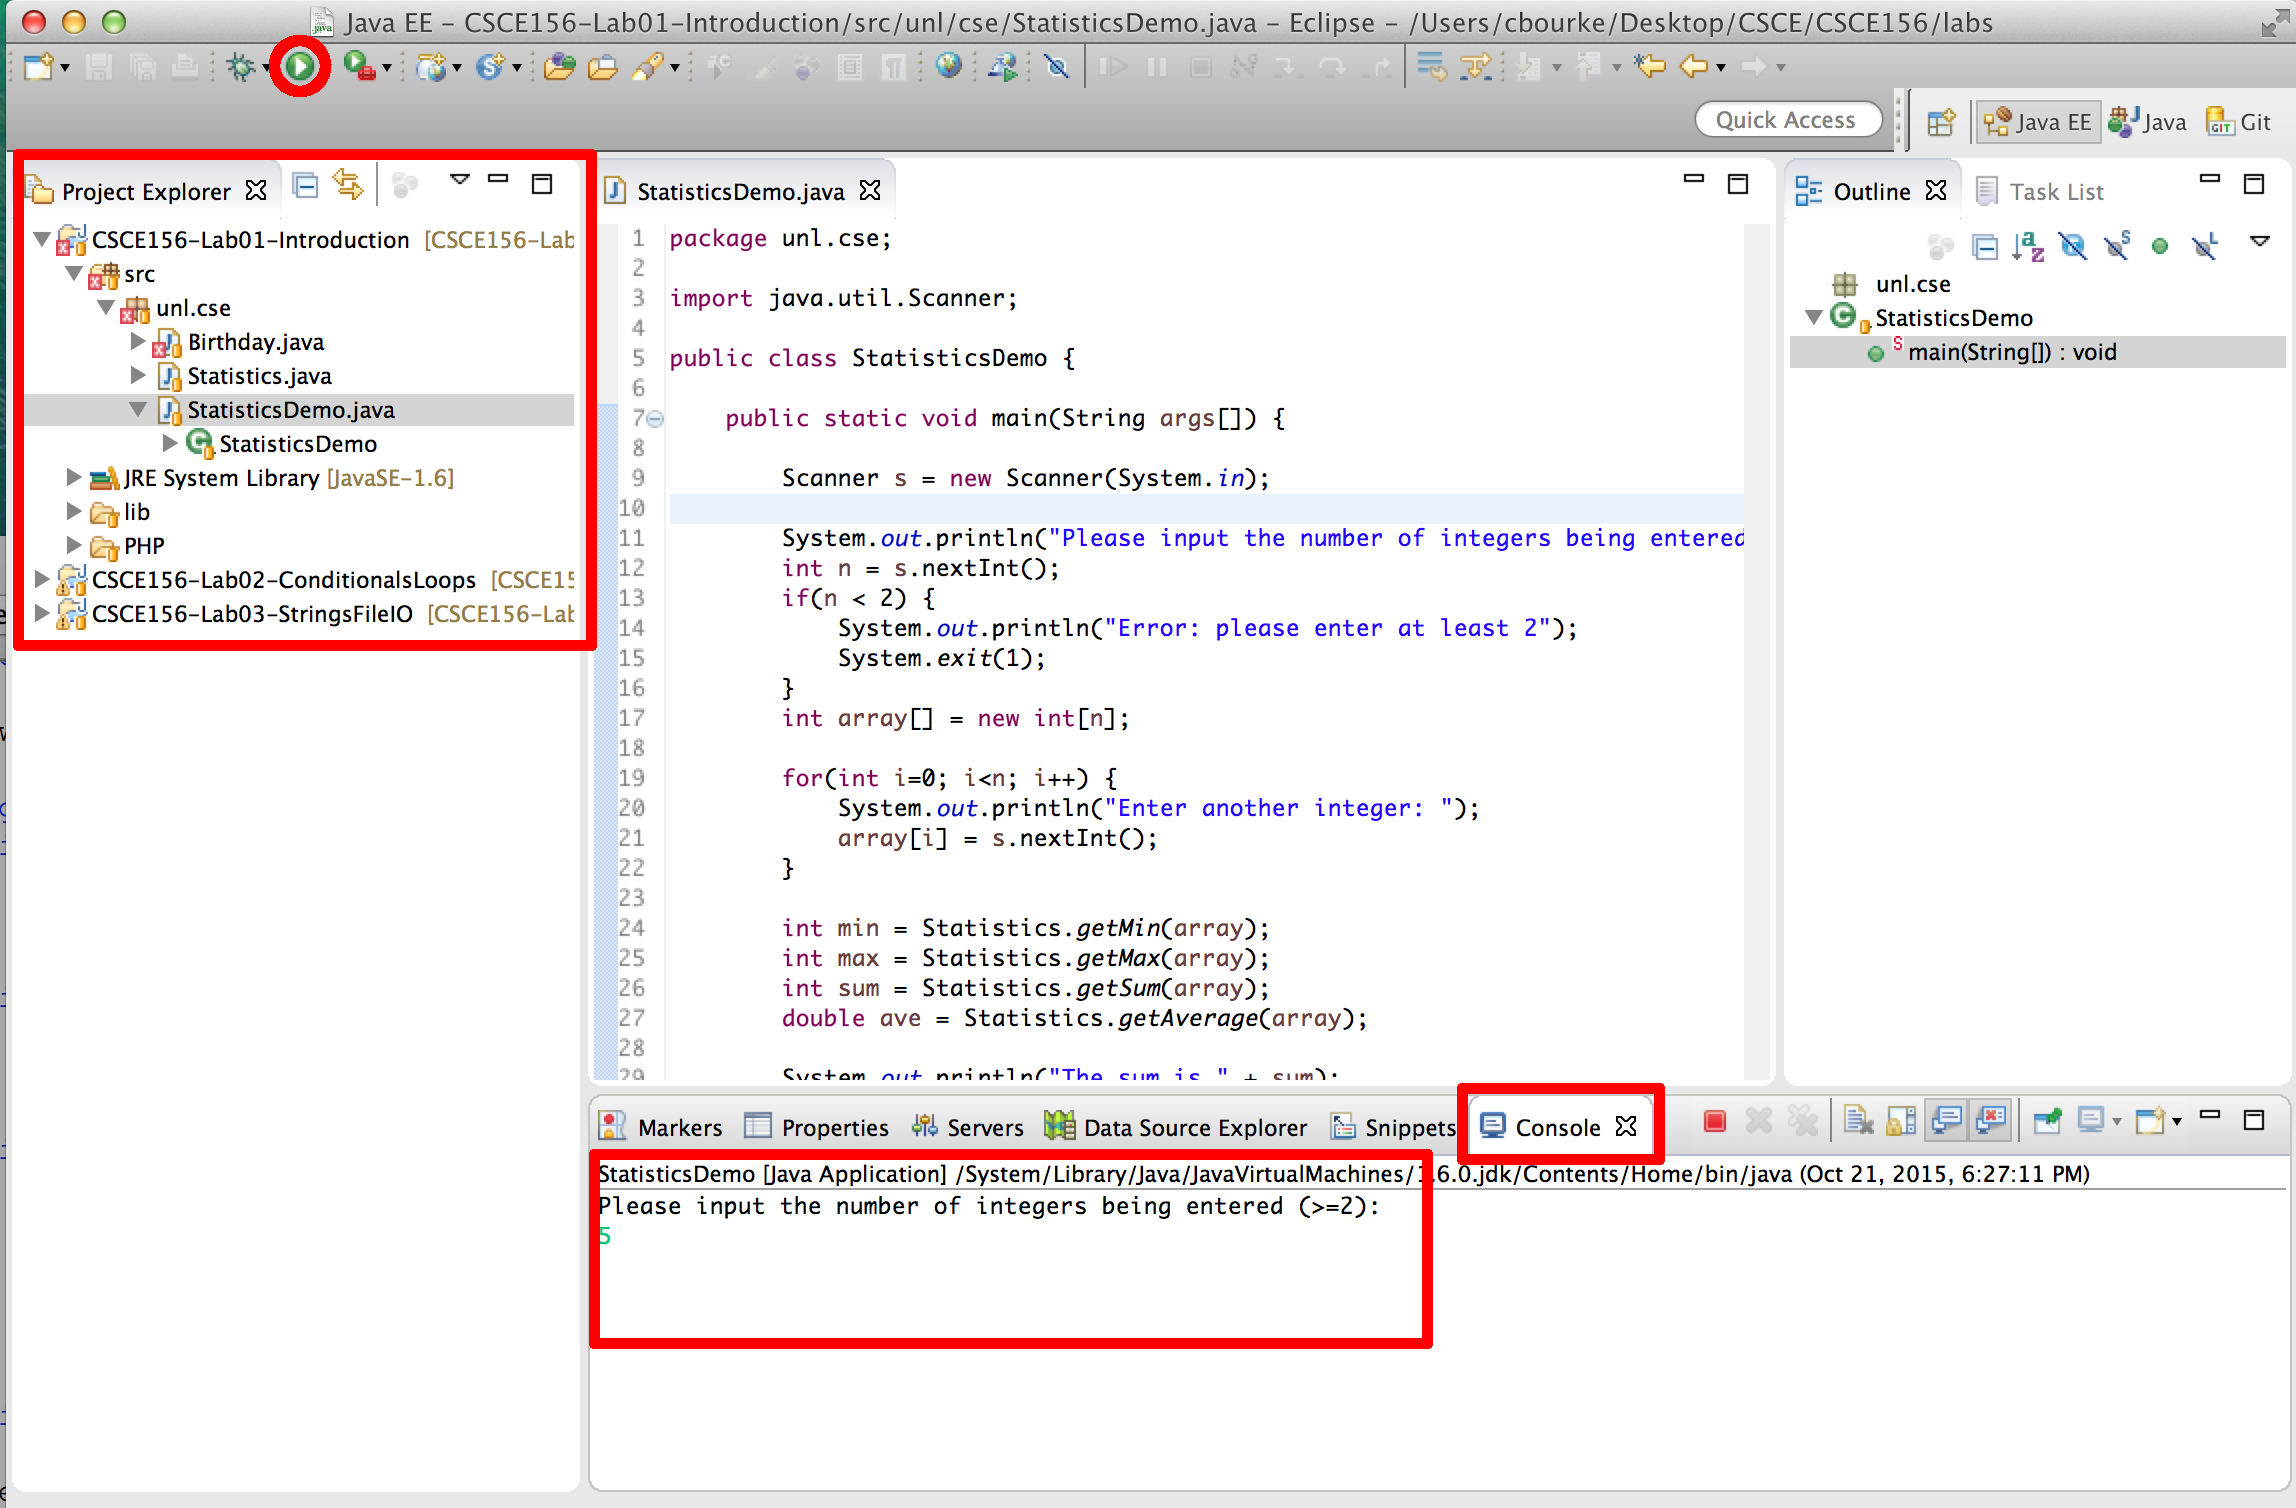
\includegraphics[scale=.35]{images/eclipseScreen}
\caption{Eclipse Screenshot, package explorer, run button, and console
input/output areas highlighted.}
\label{figure:eclipseScreen}
\end{figure}

\subsection{Completing the Statistics Program}

Though the program runs, it does not output correct answers.  You 
will need to modify these classes to complete the program.
\begin{enumerate}
  \item Implement the \mintinline{java}{getMax()} method in the 
  	\mintinline{java}{Statistics} class.  Use the \mintinline{java}{getMin()}
	method for directions on syntax.
  \item Implement the \mintinline{java}{getSum()} method in the 
  	\mintinline{java}{Statistics} class.  Use the other methods for 
	direction on syntax.
  \item Rerun the program to verify that it now works.
\end{enumerate}

\subsection{Modifying the Statistics Program}

The program you've completed is interactive in that it prompts the 
user for input.  You will now change the program to instead use command 
line arguments to read in the list of numbers directly from the command 
line.

Command line arguments are available to your main method through 
the \mintinline{java}{args} array of Strings.  The size of this array 
can be obtained by using \mintinline{java}{args.length} which is an
integer.  Modify your code to iterate through this array and convert 
the arguments to integers using the following snippet of code:

\begin{minted}{java}
for(int i=0; i<args.length; i++) {
  array[i] = Integer.parseInt(args[i]);
}
\end{minted}

The \emph{command line} may not be apparent as you are using an IDE.  
However, it is still available to you.  Instead of clicking the ``Play'' 
button to run your program, click the down arrow right next to it.  
Then select ``Run Configurations''.  This brings up a dialog box with 
which you can run custom configurations.  Click the Arguments tab and 
enter a space-delimited list of numbers under ``Program Arguments''
and click ``Run''.

\subsection{Handing In and Grading Your Program}
\label{subsection:handinGrader}

Many of your assignments will include a programming portion that will 
require you to hand in \emph{soft-copy} source files for graders to 
compile and evaluate.  To do this, you will use a web-based handin 
program.  After handing your file(s) in, you can then grade them by 
using the web grader.  To demonstrate, do the following.

\begin{enumerate}
  \item Open a browser to \url{https://cse-apps.unl.edu/handin}
  \item Login with your CSE credentials
  \item Click on this course/lab 01 and hand in the 
  	\mintinline{text}{Statistics.java} and \mintinline{text}{StatisticsDemo.java} source files.  You can
  	either click the large ``handin'' area and select the file or you 
	can drag-drop the files.  You will be able to re-handin the same 
	file as many times as you want up until the due date.
  \item Now that the file has been handed in, you can ``grade'' yourself 
  	by using the webgrader; open a new tab/window and point your browser 
	to \url{https://cse.unl.edu/~cse156/grade} (depending on your
	section, this URL may be different).
  \item Fill the form with your CSE login and password, select the 
  	appropriate assignment (Lab 01) and click ``Grade''
\end{enumerate}

For future assignments and labs, you can compare the results of 
your program with the ``Expected Results''.  If there are problems or
errors with your program(s), you should fix/debug them and repeat the
handin/grading process.  You can do this as many times as you like up 
until the due date.  Some programs and assignments will run test cases 
and may provide expected output alongside your output.  Others may 
have more sophisticated test cases and actually provide you a percentage 
of test cases passed.  It is your responsibility to read, understand 
and \emph{address} all of the errors and/or warnings that the grader 
produces.

\section{IDE Orientation}

In the next activities you'll get more familiar with using Eclipse and the
convenient functionality IDEs provide.  

\subsection{Using External Libraries}

No man is an island.  Good code depends on selecting and (re)using 
standard libraries whenever possible so that you are not continually reinventing the wheel.  This activity will familiarize you with how 
to import and use an external Java library.  Java libraries are 
usually packaged into JAR (\textbf{J}ava \textbf{AR}chive) files 
which contain a collection of compiled class files and other resources necessary to use the library.

\begin{enumerate}
  \item You'll notice that there are compilation errors in the 
  	\mintinline{text}{Birthday.java} file.  This is because this 
	class uses other classes that are not available in the standard 
	JDK (Java Development Kit).  It instead uses classes from the 
	Joda-Time library; a library of useful classes and utilities for 
	dealing with dates, times, intervals, durations, etc.
  \item The JAR file, \mintinline{text}{joda-time-2.0.jar} has
    been included in the project in the \mintinline{text}{lib} folder.
    External libraries are usually kept in a hierarchy of folders
    like this (you can create your own folders by right-clicking 
    the project and selecting ``New'' $\rightarrow$ ``Folder'')
  \item Right-click the JAR file and select ``Build Path'' $\rightarrow$ 
  	``Add to Build Path.''  The library is now included in your project
	and the compiler errors should go away.
\end{enumerate}

\subsection{Cleaning Up}

Though the syntax errors should now be resolved, the code isn't pretty
making it difficult to read and understand.  Eclipse provides a built-in
code formatter functionality.  Typically if you write good code to begin
with it will automatically provide consistent indentation and other stylistic
features.  It is best practice to get in the habit of writing good, clean
code automatically.  

However, if you need to clean up a file in one shot you can do use the
auto-formatter feature.  

\begin{itemize}
  \item On Windows: press control-shift-f to reformat the code
  \item On Mac: press shift-command-f to reformat the code
\end{itemize}

Another issue with the code is that it is using \mintinline{text}{lower_underscore_casing} for some of its variables.  Change the 
variable names to the preferred \mintinline{text}{lowerCamelCasing} 
convention in Java.  You could do this manually but a neat trick that
most IDEs provide is as follows.

\begin{enumerate}
  \item Highlight the variable name (any instance will do)
  \item Right click and select \mintinline{text}{Refactor} $\rightarrow$ \mintinline{text}{Rename}
  \item Type the new variable name and hit enter and it will automatically be changed for all instances!  
\end{enumerate}

\subsection{Finishing The Program}

Though the program should have no syntax errors, if you run it, no 
output will be displayed.  You need to complete the program as follows.

\begin{enumerate}
  \item For the variables, name, month, date, and year, enter your 
  	own information (your name and your birthday).
  \item Add appropriate code (using \mintinline{java}{System.out.println()})
    which prints to the standard output a full line) a greeting similar
    to the following. 
    
    \mintinline{text}{Greetings, NAME.  Today you are XX years, 
    XX months, and XX days old.}  
    
    Of course, the placeholders should
    be replaced with variable values.  In Java, variable values can be
    concatenated with strings using the \mintinline{java}{+} (plus) 
    operator.
  \item Add a conditional statement that, if today is the user's birthday 
    will output \mintinline{text}{Happy Birthday}.  If it is not the 
    user's birthday, output 
    
    \mintinline{text}{Your friends have XX shopping days until your next birthday} 
    
    again with an appropriate variable
    value.
  \item Complete your worksheet and demonstrate your working code to a 
  	lab instructor.
\end{enumerate}

\section*{Advanced Activity (Optional)}

Explore the Joda-Time library (its API is available at: \url{http://joda-time.sourceforge.net/api-release/index.html}) and Java itself by implementing the following program.  The program will read in (or hard code) two birthdays and compute the number of years, months, and days between them.  

\section{Running \& Editing PHP}
\label{section:phpPart}

The project you checked out from GitHub contains a \mintinline{text}{PHP}
folder in which there are several PHP scripts.  We will now familiarize
you with editing and running these scripts.  These instructions assume
that you are working on a lab computer.  You may work on your own 
machine, but you will need to install a PHP interpreter or an SSH client 
such as Putty.

The PHP file, \mintinline{text}{statistics.php} contains a PHP program 
that prompts the user to enter a number of integers and computes several 
statistics (minimum, maximum, average, sum) and outputs the results.  
Most of the program's framework has been provided for you.  In this 
activity, you will write the remainder of the program.

\begin{enumerate}
  \item Review the \mintinline{text}{statistics.php} code in Eclipse or
    the text editor of your choice.
  \item Login to CSE account using SSH or Putty.  You can execute your 
  	script using PHP's Command Line Interface (CLI) as follows:
	
    \mintinline{text}{php statistics.php}
	
  \item Though the script runs, it does not output the correct values.  
	To get it to work, you will need to implement the following two 
	functions:
	\begin{itemize} 
	  \item \mintinline{php}{getMax($array)} -- This method should 
	  return the maximum of the elements in the array.
      \item \mintinline{php}{getSum($array)} -- This method should 
	  return the sum of the elements in the array.
	\end{itemize}
  \item Rerun your program to check that it works.
\end{enumerate}

\subsection{Modifying The Script}

The program you've completed is interactive in that it prompts the 
user for input.  You will now change the script to instead use 
command line arguments to read in the list of numbers directly 
from the command line.

PHP supports command line arguments by providing a built-in array, 
\mintinline{php}{$argv} which is 0-indexed.  Note: the first element 
in this array is the script's name, so you will need to process 
starting from index 1.  Once you have made the appropriate changes, 
you should be able to execute your script as follows:

\mintinline{text}{php statistics.php 10 20 30 40}

\subsection{Submitting and Grading Your Program}

Go to section \ref{subsection:handinGrader} and follow the instructions
to submit and grade your script.

\section{PHP in a Dynamic Webpage}

You will now utilize PHP in a dynamic, interactive web page.  The 
webserver is responsible for handling requests from clients 
(browsers), executing the proper PHP script(s) and returning the 
output (HTML) to the client.  This activity will have you finishing 
two PHP pages that reads a user's name and birthday and tells them 
how old they are.

\begin{enumerate}
  \item The Apache webserver on CSE has been setup so that each user 
  	can place files into a \mintinline{text}{public_html} directory 
	and these files will be available through a web browser.  To
	create this directory, use the following command (in Putty):

	\mintinline{text}{mkdir public_html}
	
  \item Make sure your \mintinline{text}{public_html} directory 
	world executable using this command:
	
	\mintinline{text}{chmod go+x public_html}

  \item Copy the \mintinline{text}{birthday.php} and 
  	\mintinline{text}{birthday_result.php} files into your 
	\mintinline{text}{public_html} directory and make them 
	world-readable using the command:
	
	\mintinline{text}{chmod o+r *.php}
	
  \item Open a web browser using the URL, 
  	\url{http://cse.unl.edu/~login/birthday.php} with 
	\mintinline{text}{login} replaced with your login.
	You will need to modify the scripts to get them working
  	properly.  
\end{enumerate}

The \mintinline{text}{birthday.php} page should render in your web 
browser without any problems.  However, it is incomplete.  Take 
these steps to get it in working order.

\begin{enumerate}
  \item There are several months missing from the drop 
  	down menu.  Include them by modifying the code that builds 
	the \mintinline{text}{$month} array.
  \item Modify the code as indicated to populate the Date drop 
	down menu so that dates 1 thru 31 appear.  Use the year drop 
	down menu as a model.
\end{enumerate}
	
The HyperText Transfer Protocol (HTTP) allows clients to 
\mintinline{text}{POST} data to another page for processing.  
You'll notice that your HTML form in the birthday.php is 
configured to post its results to \mintinline{text}{birthday_result.php}.  
Parameters posted to this page are specified by the input elements 
in the HTML form using the name property.  In the result page, 
these parameters are available through the \mintinline{php}{$_POST} 
array.  This is an associative array (indexed by strings).  
You can get the posted values using the syntax, 
\mintinline{php}{$name = $_POST['name'];} where \mintinline{php}{'name'}
is replaced with the name of the form value.

\begin{enumerate}
  \item Modify the result page to pull the values posted from 
  	the form page.
  \item Also modify the script as indicated to print the appropriate 
	message.  If today is the user's birthday, print 
	\mintinline{text}{Happy Birthday!}, otherwise print 
	
	\mintinline{text}{Your friends have XX shopping days until your next birthday} 
	
	where XX is the appropriate variable value.  Note: strings can 
	be concatenated with variable values in PHP by using the period 
	operator.  An example:
	
	\mintinline{php}{print "This is PHP, version " . $version . ", have fun!";}

  \item Answer the questions in your worksheet and show your completed
  	programs to a lab instructor.
\end{enumerate}

\section*{Advanced Activity (Optional)}

Enter an invalid birthdate into your web page and observe 
what happens.  Is this behavior ideal?  Think about some 
alternatives to handle invalid dates.

Most web pages utilize some JavaScript or JavaScript frameworks 
or libraries to make the web page dynamic.  Dates are usually 
entered by having a calendar-like popup appear and have the 
users click actual dates on the calendar.  This provides a 
much better user experience and has the added benefit of 
preventing invalid dates.  

Familiarize yourself with jQuery and in particular, the ``Datepicker'' 
jQuery UI plugin (see \url{http://jqueryui.com/demos/datepicker/#dropdown-month-year}) and integrate it into your PHP page.  Note: 
changes will need to be made to both the input and the 
result page.


\end{document}
